\documentclass[11pt, twoside, pdftex]{article}

% This include all the settings that we should use for the document
\newcommand{\PDFTitle}{Debugging of Application Programs on Intel's DE-Series Boards}
\newcommand{\commonPath}{../../Common}
\newcommand{\datePublished}{Mar 2022}

\newcommand{\versnum}{21.1} %version number quartus/AMP
\newcommand{\quartusname}{Quartus\textsuperscript{\textregistered} Prime}	
\newcommand{\textBar}{For \quartusname{} \versnum{}}
\newcommand{\thisyear}{2022 } %for copyright
\newcommand{\company}{FPGAcademy.org}
\newcommand{\longteamname}{FPGAcademy.org}
\newcommand{\teamname}{FPGAcademy}
\newcommand{\website}{FPGAcademy.org}

\newcommand{\productAcronym}{AMP}
\newcommand{\productNameShort}{Monitor Program}

\newcommand{\productNameMedTM}{Monitor Program}
\newcommand{\productNameMed}{Monitor Program}

%\newcommand{\headerLogoFilePath}[1]{#1/FPGAcademy.png}



\setlength\topmargin{-0.25in}
\setlength\headheight{0in}
\setlength\headsep{0.35in}
\setlength\textheight{8.5in}
\setlength\textwidth{7in}
\setlength\oddsidemargin{-0.25in}
\setlength\evensidemargin{-0.25in}
\setlength\parindent{0.25in}
\setlength\parskip{0in} 

\pdfpagewidth 8.5in
\pdfpageheight 11in

% listings is a package that supports encapsulating source code in LaTeX conveniently

\usepackage{listings}
% add support for graphics
\usepackage{graphicx}
\usepackage[usenames, dvipsnames]{color}

\def\expandparam\lstinputlisting[#1]#2{\edef\tmp{\noexpand\lstinputlisting[#1]{#2}}\tmp}

\widowpenalty 10000
\clubpenalty 10000

%%%%%%%%%%%%%%%%%%%% Source Code Formatting %%%%%%%%%%%%%%%%%%%%
\definecolor{globalCommentColour}{rgb}{0.588,0.588,0.588}

%%%%%%%%%%%%%%%%%%%%%%%%%%%%%%%%%%%%%%%%%%%%%%%%%%%%
% Defining a NiosII ASM highlighter for lstlisting
\lstdefinelanguage[NiosII]{Assembler} {
 	morekeywords={add, addi, and, andhi, andi, beq, bge, bgeu, bgt, bgtu, ble,  bleu, blt, bltu, bne, br, break,% 
 	bret, call, callr, cmpeq, cmpeqi, cmpge, cmpgei, cmpgeu, cmpgeui, cmpgt, cmpgti, cmpgtu, cmpgtui, cmple,%
 	cmplei, cmpleu, cmpleui, cmplt, cmplti, cmpltu, cmpltui, cmpne, cmpnei, custom, div, divu, eret, flushd,%
 	flushda, flushi, flushp, initd, initda, initi, jmp, jmpi, ldb, ldbio, ldbu, ldbuio, ldh, ldhio, ldhu, ldhuio,%
 	ldw, ldwio, mov, movhi, movi, movia, movui, mul, muli, mulxss, mulxsu, mulxuu, nextpc, nop, nor, or, orhi, ori,%
 	rdctl, rdprs, ret, rol, roli, ror, sll, slli, sra, srai, srl, srli, stb, stbio, sth, sthio, stw, stwio,%
 	sub, subi, sync, trap, wrctl, wrtcl, wrprs, xor, xori, xorhi, xori},% 	
 	morekeywords=[2]{.abort, .ABORT, .align, .app-file, .ascii, .asciz, .balign, .byte, .comm, .data, .def,%
 	.desc, .dim, .double, .eject, .else, .end, .endef, .endif, .equ, .equiv, .err, .extern, .file, .fill, .float,%
 	.global, .globl, .hword, .ident, .if, .include, .int, .irp, .irpc, .lcomm, .lflags, .line, .linkonce, .ln,%
 	.list, .long, .macro, .mri, .nolist, .octa, .org, .p2align, .psize, .quad, .rept, .sbttl, .scl, .section,%
 	.set, .short, .single, .size, .sleb128, .skip, .space, .stadb, .stabn, .stabs, .string, .symver, .tag,%
 	.text, .title, .type, .val, .uleb128, .word},% 	
 	morekeywords=[3]{et, bt, gp, sp, fp, ea, sstatus, ra, pc, status, estatus, bstatus, ienable, ipending, cpuid,%
 	exception, pteaddr, tlbacc, tlbmisc, eccinj, badaddr, config, mpubase, mpuacc},% 	
 	sensitive=t,%
 	alsoletter=.,%
	morestring=[b]",%
 	morecomment=[s]{/*}{*/},%
 	morecomment=[l]\#,%
   }[keywords,comments,strings]
   
   %% NOTE: morekeywords=[2] are GNU directives.
   
   \definecolor{niosInstructionColour}{rgb}{0.000,0.608,0.000}
   \definecolor{niosDirectiveColour}{rgb}{0.000,0.000,0.902}
   \definecolor{niosSpecialRegColour}{rgb}{0.000,0.000,0.000}
   \definecolor{niosStringColour}{rgb}{0.808,0.482,0.000}
   
   %% NOTE: To make bold use: =\bfseries\color{<colour>}
   \lstdefinestyle{defaultNiosStyle} {
   language=[NiosII]{Assembler},
   stringstyle=\color{niosStringColour},
   keywordstyle=\color{niosInstructionColour},
   keywordstyle=[2]\color{niosDirectiveColour},
   keywordstyle=[3]\itshape\color{niosSpecialRegColour}
   }
%%%%%%%%%%%%%%%%%%%%%%%%%%%%%%%%%%%%%%%%%%%%%%%%%%%%

%%%%%%%%%%%%%%%%%%%%%%%%%%%%%%%%%%%%%%%%%%%%%%%%%%%%
% Defining a ArmA9 ASM highlighter for lstlisting
\lstdefinelanguage[ArmA9]{Assembler} {
 	morekeywords={ADC, ADD, ADDS, AND, ANDS, B, BAL, BEQ, BGE, BGT, BL, BLT, BIC, BKPT, BLX, BNE, BX, CDP, CLZ, CMN, CMP, EOR,%
 	EORS, LDC, LDM, LDR, LDRB, LDRBT, LDRH, LDRSB, LDRSH, LDRT, LSL, MCR, MLA, MOV, MOVW, MOVT, MRC, MRS, MSR, MUL, MVN, ORR, PLD,%
 	ROR, RSB, RSC, SBC, SMLAL, SMULL, STC, STM, STR, STRB, STRBT, STRH, STRT, SUB, SUBS, SWI, SWP, SWPB, TEQ, UMLAL,
 	PUSH, POP, MOVS, RORS, LSR},%
 	morekeywords=[2]{.abort, .ABORT, .align, .app-file, .ascii, .asciz, .balign, .byte, .comm, .data, .def,%
 	.desc, .dim, .double, .eject, .else, .end, .endef, .endif, .equ, .equiv, .err, .extern, .file, .fill, .float,%
 	.global, .globl, .hword, .ident, .if, .include, .int, .irp, .irpc, .lcomm, .lflags, .line, .linkonce, .ln,%
 	.list, .long, .macro, .mri, .nolist, .octa, .org, .p2align, .psize, .quad, .rept, .sbttl, .scl, .section,%
 	.set, .short, .single, .size, .sleb128, .skip, .space, .stadb, .stabn, .stabs, .string, .symver, .tag,%
 	.text, .title, .type, .val, .vectors, .uleb128, .word},%
 	morekeywords=[3]{SP, PC, MIDR, CTR, TCMTR, TLBTR, MPIDR, ID_PFR0, ID_PFR1, ID_DFR0, ID_MMFR0, ID_MMFR1, ID_MMFR2,%
 	ID_MMFR3, ID_ISAR0, ID_ISAR1, ID_ISAR2, ID_ISAR3, ID_ISAR4, CCSIDR, CLIDR, AIDR, CSSELR, TTBR0, TTRB1, TTBR2, DACR,%
 	DFSR, IFSR, ADFSR, AIFSR, DFAAR, IFAR, ICIALLUIS, BPIALLIS, PAR, ICIALLU, ICIMVAU, BPIALL, DCIMVAC, DCISW, V2PCWPR,%
 	DCCVAC, DCCSW, DDIMVAC, DCISW, TLBALLIS, TLBIMVAIS, TLBIASIDIS, TLBIMVAAIS, TLBIALL, TLBIMVA, TLBIASID, TLBIMVAA,%
 	PMCR, PMCNTENSET, PMCNTENCLR, PMOVSR, PMSWINC, PMSELR, PMXEVTYPER, PMXEVCNTR, PMUSERENR, PMINTENSET, PMINTENCLR,%
 	PRRR, NRRR, PLEIDR, PLEASR, PLEFSR, PLEUAR, PLEPCR, VBAR, MVBAR, ISR, FCSEIDR, CONTEXTIDR, TPIDRURW, TPIDRURO, TPIDRPRW},%
 	sensitive=f,%
 	alsoletter=.,%
	morestring=[b]",%
 	morecomment=[s]{/*}{*/},%
 	morecomment=[l]{//},%
   }[keywords,comments,strings]
   
   %% NOTE: morekeywords=[2] are GNU directives.
   
   \definecolor{armInstructionColour}{rgb}{0.000,0.608,0.000}
   \definecolor{armDirectiveColour}{rgb}{0.000,0.000,0.902}
   \definecolor{armSpecialRegColour}{rgb}{0.000,0.000,0.000}
   \definecolor{armStringColour}{rgb}{0.808,0.482,0.000}
   
   \lstdefinestyle{defaultArmStyle} {
   language=[ArmA9]{Assembler},
   stringstyle=\color{armStringColour},
   keywordstyle=\color{armInstructionColour},
   keywordstyle=[2]\color{armDirectiveColour},
   keywordstyle=[3]\itshape\color{armSpecialRegColour}
   }
%%%%%%%%%%%%%%%%%%%%%%%%%%%%%%%%%%%%%%%%%%%%%%%%%%%%

%%%%%%%%%%%%%%%%%%%%%%%%%%%%%%%%%%%%%%%%%%%%%%%%%%%%
% Defining style for the verilog.

\definecolor{verilogCommentColour}{rgb}{0.000,0.502,0.000}

\lstdefinestyle{defaultVerilogStyle} {
language={Verilog},
keywordstyle=\color{blue},
commentstyle=\color{verilogCommentColour}
}
%%%%%%%%%%%%%%%%%%%%%%%%%%%%%%%%%%%%%%%%%%%%%%%%%%%%

%%%%%%%%%%%%%%%%%%%%%%%%%%%%%%%%%%%%%%%%%%%%%%%%%%%%
% Defining style for the vhdl.
\lstdefinestyle{defaultVHDLStyle} {
language={VHDL},
keywordstyle=\color{blue},
commentstyle=\color{verilogCommentColour}
}
%%%%%%%%%%%%%%%%%%%%%%%%%%%%%%%%%%%%%%%%%%%%%%%%%%%%

%%%%%%%%%%%%%%%%%%%%%%%%%%%%%%%%%%%%%%%%%%%%%%%%%%%%
% Java
\definecolor{javaStringColour}{rgb}{0.808,0.482,0}
%%%%%%%%%%%%%%%%%%%%%%%%%%%%%%%%%%%%%%%%%%%%%%%%%%%%

%%%%%%%%%%%%%%%%%%%%%%%%%%%%%%%%%%%%%%%%%%%%%%%%%%%%
% Defining language styles
% C
\definecolor{CStringColour}{rgb}{0.808,0.482,0}
%%%%%%%%%%%%%%%%%%%%%%%%%%%%%%%%%%%%%%%%%%%%%%%%%%%%

%%%%%%%%%%%%%%%%%%%%%%%%%%%%%%%%%%%%%%%%%%%%%%%%%%%%
% Defining extended LaTeX language.
\lstdefinelanguage[LocalLaTeX]{TeX}[LaTeX]{TeX}%
 	{moretexcs={bf, it, sf, lstset},%
   	}%

\lstdefinestyle{defaultLocalLatexStyle} {
language=[LocalLatex]{TeX},
keywordstyle=\color{blue}\bfseries,
keywordstyle=[2]\color{blue},
keywordstyle=[3]\color{blue}\bfseries
}
%%%%%%%%%%%%%%%%%%%%%%%%%%%%%%%%%%%%%%%%%%%%%%%%%%%%

\lstset{
%language = C,
%language = Verilog,
%basicstyle=\color{black}\rmfamily\ttfamily,
basicstyle=\small\color{black}\ttfamily,
commentstyle=\small\color{globalCommentColour}\itshape\ttfamily,
keywordstyle=\small\color{blue}\bfseries\ttfamily,
showstringspaces=false,
frame=none, %lines % boxed listings
breaklines=true,
breakatwhitespace=true,
tabsize=4
}
%%%%%%%%%%%%%%%%%%%%%%%%%%%%%%%%%%%%%%%%%%%%%%%%%%%%%%%%%%%%%%%%


%\usepackage[centering]{geometry}.
%%%%%%%%%%%%%%%%%%%%%%%%%%%%%%%%%%%%%%%%%%%%%%%%%%%
% Document Settings
\usepackage[labelsep=period]{caption}
% we can choose a better font later
%\usepackage{palatino}
\usepackage{fourier}
%\fontencoding{T1}
% include common used symbols
\usepackage{textcomp}
% add support for graphics
\usepackage{graphicx}
\usepackage[usenames, dvipsnames]{color}
% enable to draw thick or thin table hlines
\setlength{\doublerulesep}{\arrayrulewidth}
\usepackage{longtable}
\setlongtables
%\usepackage{array}
% It may be better to use PDFLaTeX as it can generate bookmarks for the
% document

% Add some useful packages
\usepackage{ae,aecompl}
\usepackage{epsfig,float,times}

% reset the font for section
\usepackage{sectsty}
%\allsectionsfont{\fontfamily{ptm}\selectfont}
\allsectionsfont{\usefont{OT1}{phv}{bc}{n}\selectfont}

% use compact space for sections
\usepackage[compact]{titlesec}
\titlespacing{\section}{0pt}{0.2in}{*0}
\titlespacing{\subsection}{0pt}{0.1in}{*0}
\titlespacing{\subsubsection}{0pt}{0.05in}{*0}

% fancyhdr header and footer customization
\usepackage{layout}
\usepackage{fancyhdr}
\pagestyle{fancy}
\fancyhead{}
\fancyhead[R]{\textit{\tiny{\textBar}}}
\fancyfoot{}
\fancyfoot[LO,
RE]{\textrm{\href{https://www.fpgacademy.org}{\small \longteamname}} \\ {\small \datePublished }}
\fancyfoot[RO, LE]{\small \thepage}
% two-side settings
%\fancyhead{} % clear all header fields
%\fancyfoot{} % clear all footer fields
%\fancyfoot[LE,RO]{\thepage}
\renewcommand{\headrulewidth}{2pt}
\renewcommand{\headrule}{{\color{blue} \hrule width\headwidth height\headrulewidth \vskip-\headrulewidth}}
\renewcommand{\footrulewidth}{0pt}

% Format the footer on page 1
\fancypagestyle{plain}{
\fancyhead{}
\fancyfoot{}
\fancyfoot[LO,
RE]{\textrm{\href{https://www.fpgacademy.org}{\small \longteamname}} \\ {\small \datePublished }}
\fancyfoot[RO, LE]{\small \thepage}
\renewcommand{\headrulewidth}{0pt}
}
% adjust some setting to try to make the figure stay in the same page with text
% Reference: 	http://www.cs.uu.nl/~piet/floats/node1.html
%   			http://mintaka.sdsu.edu/GF/bibliog/latex/floats.html
%   General parameters, for ALL pages:
\renewcommand{\topfraction}{0.9}	% max fraction of floats at top
\renewcommand{\bottomfraction}{0.8}	% max fraction of floats at bottom
%   Parameters for TEXT pages (not float pages):
\setcounter{topnumber}{3}
\setcounter{bottomnumber}{3}
\setcounter{totalnumber}{5}     % 2 may work better
\setcounter{dbltopnumber}{2}    % for 2-column pages
\renewcommand{\dbltopfraction}{0.9}	% fit big float above 2-col. text
\renewcommand{\textfraction}{0.07}	% allow minimal text w. figs
%   Parameters for FLOAT pages (not text pages):
\renewcommand{\floatpagefraction}{0.7}	% require fuller float pages
% N.B.: floatpagefraction MUST be less than topfraction !!
\renewcommand{\dblfloatpagefraction}{0.7}	% require fuller float pages
%%%%%%%%%%%%%%%%%%%%%%%%%%%%%%%%%%%%%%%%%%%%%%%%%%%
% remember to use [htp] or [htpb] for placement
%%%%%%%%%%%%%%%%%%%%%%%%%%%%%%%%%%%%%%%%%%%%%%%%%%%

% set no indent for paragraph
\setlength{\parindent}{0em}
\addtolength{\parskip}{11pt}
\newcommand{\compact}{[topsep=0pt]}
% use this package to reduce space
\usepackage{enumitem}
\usepackage{multirow}
\usepackage{rotating}
\usepackage{pifont}
\usepackage{dingbat}
\newcommand{\itemsecond}{$\circ$}
%
%%%%%%%%%%%%%%%%%%
\date{}
\author{}
%%%%%%%%%%%%%%%%%%
\newcommand{\de}{DE-series}
\newcommand{\up}{FPGAcademy}
\newcommand{\fabric}{Avalon Switch Fabric}
\newcommand{\TODO}[1]{\textcolor{red}{\textbf{TODO}: #1}}
\def\registered{{\ooalign{\hfil\raise .00ex\hbox{\scriptsize R}\hfil\crcr\mathhexbox20D}}}

% enable url and reference(bookmarks) in pdf
\usepackage{url}
\usepackage[pdftex, colorlinks]{hyperref}
\hypersetup{%
pdftitle={\PDFTitle},
linkcolor=blue,
hyperindex=true,
pdfauthor={\longteamname},
pdfkeywords={FPGAcademy, Academic Program, Example System},
bookmarksnumbered,
bookmarksopen=false,
filecolor=blue,
pdfstartview={FitH},
urlcolor=blue,
plainpages=false,
pdfpagelabels=true,
linkbordercolor={1 1 1} %no color for link border
}%
%%%%%%%%%%%%%%%%%%%%%%%%%%%%%%%%%%%%%%%%%%%%%%%%%%%
\setlength{\fboxsep}{0.7pt}
\setlength{\fboxrule}{0.5pt}

\newcommand{\red}[1]{{\color{red}\sf{#1}}}
\newcommand{\blue}[1]{{\color{blue}\sf{#1}}}



%%%%%%%%%%%%%%%%%%%%%%%%%
% Add title
\newcommand{\doctitle}{Debugging of Application Programs \\ on Intel's DE-Series Boards}
\newcommand{\dochead}{Debugging of Application Programs on Intel's DE-Series Boards}
% Usually no need to change these two lines
\title{\fontfamily{phv}\selectfont{\doctitle} }
\chead{ \small{\textsc{\bfseries \dochead} } }
% Customizations
%%%%%%%%%%%%%%%%%%%%%%%%%
% Allows multiple figures per page

\renewcommand\floatpagefraction{.9}
\renewcommand\topfraction{.9}
\renewcommand\bottomfraction{.9}
\renewcommand\textfraction{.1}   
\setcounter{totalnumber}{50}
\setcounter{topnumber}{50}
\setcounter{bottomnumber}{50}
\widowpenalty 10000
\clubpenalty 10000
\raggedbottom

%%%%%%%%%%%%%%%%%%
%%% DOCUMENT START
%\begin{document}
\begin{document}
\begin{table}
    \centering
    \begin{tabular}{p{5cm}p{4cm}}
        \hspace{-3cm}
        &
        \raisebox{1\height}{\parbox[h]{0.5\textwidth}{\Large\fontfamily{phv}\selectfont{\textsf{\doctitle}}}}
    \end{tabular}
    \label{tab:logo}
\end{table}

\colorbox[rgb]{0,0.384,0.816}{\parbox[h]{\textwidth}{\color{white}\textsf{\textit{\textBar}}}}

\thispagestyle{plain}
 
\section{Introduction}

This tutorial presents some basic concepts that can be helpful
in debugging of application programs written in the Nios\textsuperscript{\textregistered} II assembly language,
which run on the Intel\textsuperscript{\textregistered} DE-series boards. A simple illustrative example involves the \productNameMed{} software used to compile, 
load and run the example assembly language code on the Nios II processor with a DE-series board.

The reader is expected to be familiar with the Nios II processor, 
as well as the \productNameMed{}.
An introduction to this software is provided in tutorials:
{\it Introduction to the Intel Nios II Soft Processor}
and {\it \productNameMed{}},
which can be found in the University Program section of the web site.

{\bf Contents}:
\begin{itemize}
\item Example Circuit
\item Debugging Concepts
\item Corrective Action
\item Finding Errors in an Application Program
\item Concluding Remarks
\end{itemize}
\clearpage
\newpage

\section{Background}

Designers of digital systems are inevitably faced with the task of debugging their
imperfect initial designs. This task becomes more difficult as the system grows in
complexity. The debugging process requires determination of possible flaws in the
designed circuits as well as the flaws in application programs that are supposed to
run on this hardware. This tutorial addresses the second of these aspects of debugging.
A discussion of hardware debugging is available in the tutorial
{\it Debugging of Hardware Designs on DE-Series Boards}.

\begin{figure}[h!]
   \begin{center}
        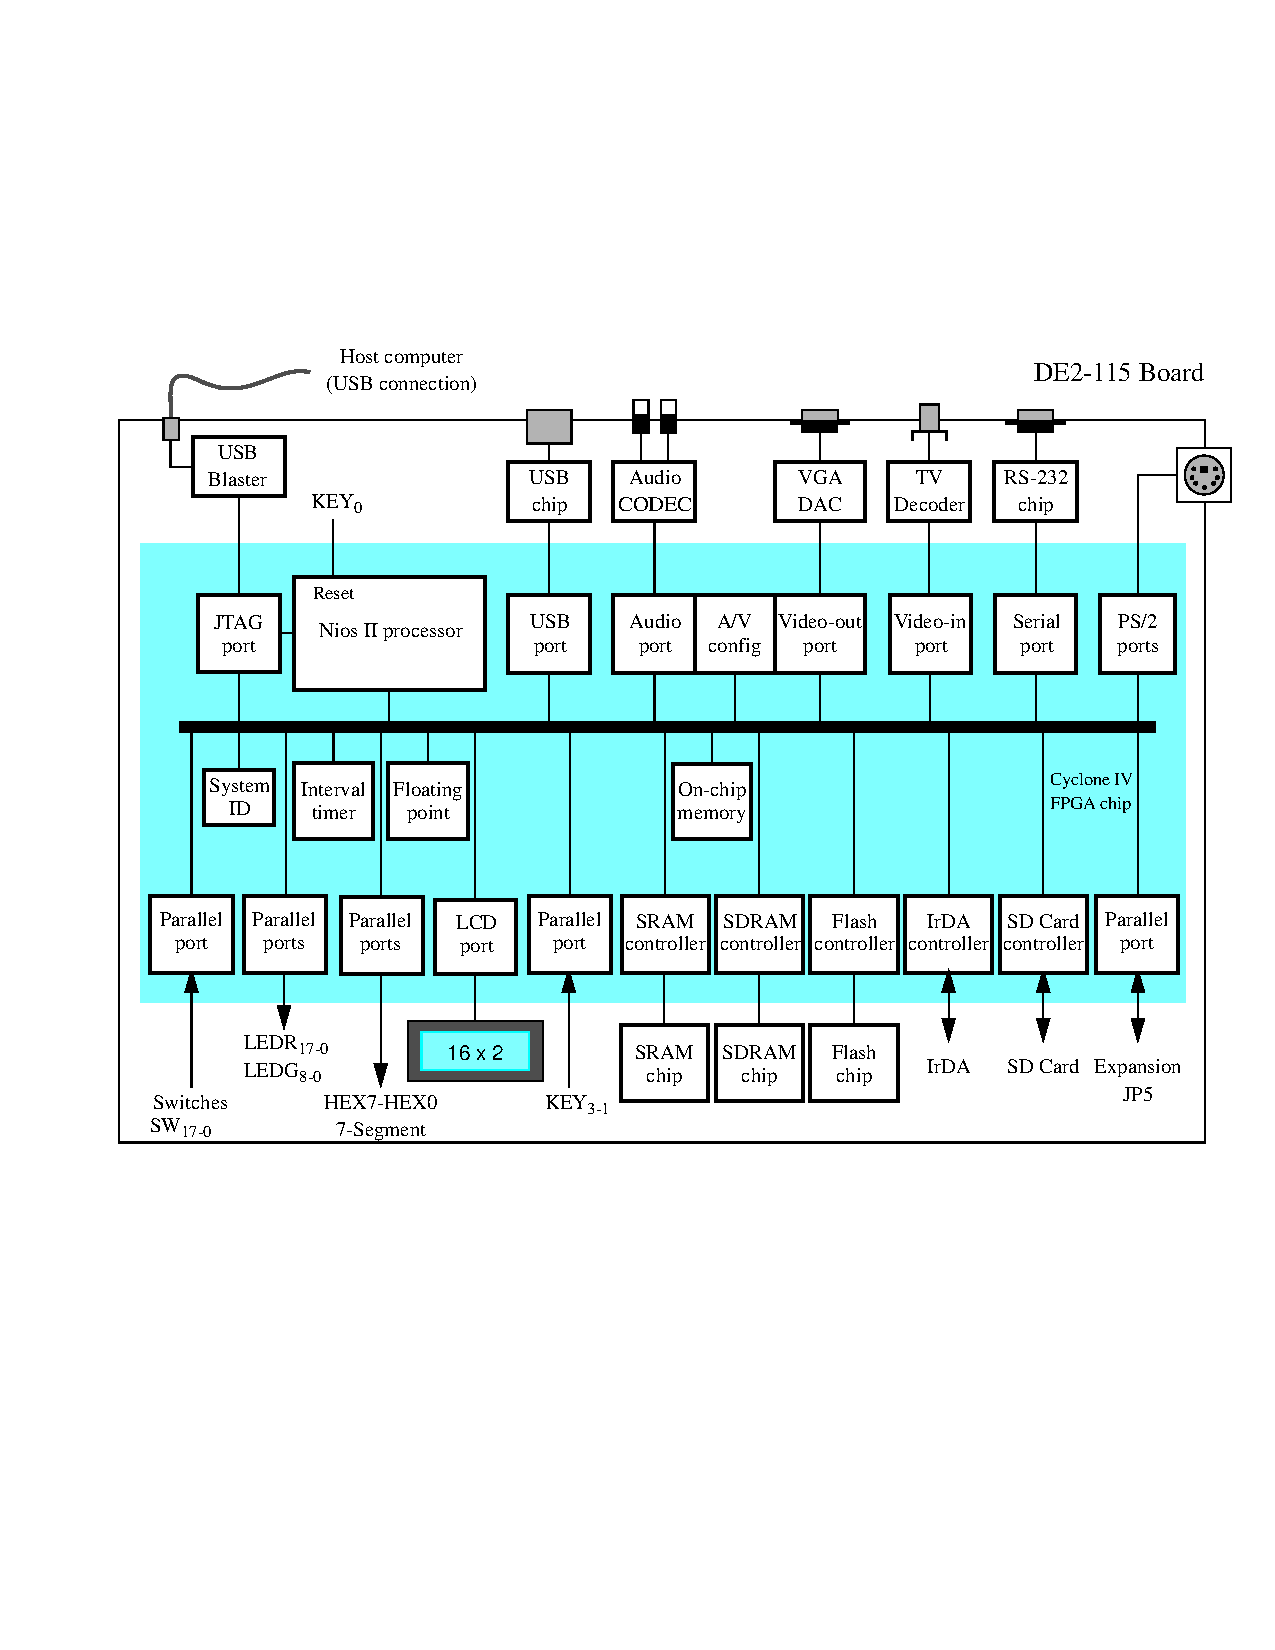
\includegraphics[scale=0.80]{figures/fig_block_diagram.pdf}
   \end{center}
   \caption{Block diagram of the DE2-115 Computer System.}
	\label{fig:1}
\end{figure}

\section{Example System}
Our example system is the DE2-115 Computer System that can be used to test the reaction time of a person
to a visual stimulus. The user initiates the test by pressing a pushbutton key, 
{\it KEY}$_1$. After some delay (of at least one second) the circuit turns on a light. 
In response, the user presses any one of {\it KEY}$_3$ to {\it KEY}$_1$, as quickly as possible, which 
results in turning the light off and displaying the elapsed time in
hundredths of a second on the 7-segment displays 
on the DE-series board. A block diagram and Platform Designer implementation of the system for the DE2-115 board is given in Figure~\ref{fig:1} and Figure~\ref{fig:2}, respectively.

The computer system for the other DE-series boards varies only where a given peripheral does not exist or is of a different size. See the computer system documentation for your specific board for more information.
 
\begin{figure}[H]
   \begin{center}
      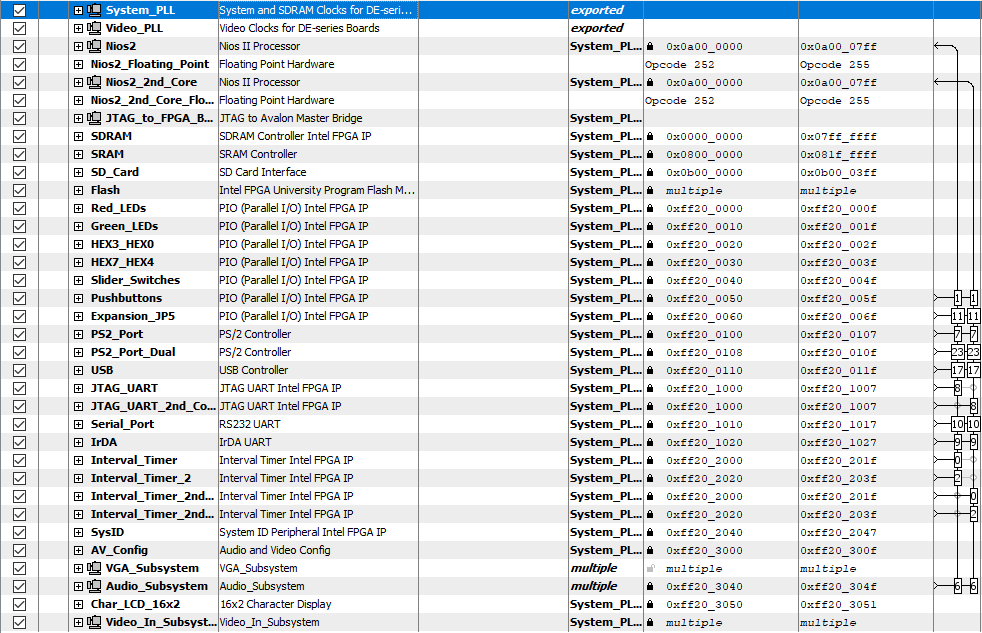
\includegraphics[scale=0.6]{figures/figure2.png}
   \caption{The system defined in the Platform Designer tool.} 
	 \label{fig:2}
	 \end{center}
\end{figure}

The processor is Nios II/s and the application is loaded from SDRAM.
The following key components and PIO interfaces are implemented:
\begin{itemize}
\item {\it Pushbuttons} is a multi-bit input port that reacts to the falling edge of the
input signal by setting to 1 a corresponding bit in its {\it edge-capture register}; 
{\it KEY}$_1$ (bit1) is used as the button to start the test and is configured in software to raise an interrupt when pressed.
\item {\it Green\_LEDs} is a multi-bit output port that drives the green LED
that tells the user to react.
\item {\it Interval\_Timer} is a 32-bit interval timer with a writable period and will be used to measure the reaction time.
\end{itemize}
\noindent
The addresses assigned to the PIO interfaces and interval timer are as indicated in Figure~\ref{fig:2}. A possible application program, written in the Nios II assembly language,
is presented in Figure~\ref{fig:3}. Note that we have numbered the 
statements to make it easy to refer to them in the discussion below.
The main program sets up the stack and enables interrupts to be raised by the interval timer and the {\it Pushbuttons} PIO. It also sets up the processor to allow interrupts. Finally, it enters 
a loop continuously checking the status of the start flag before it begins the test.
%\lstinputlisting[style=defaultNiosStyle, numbers=left, stepnumber=1]{app_software/reaction_tester.s}
\begin{figure}[H]
\begin{center}
\lstinputlisting[style=defaultNiosStyle, numbers=left, stepnumber=1, lastline=41]{app_software/reaction_tester.s}
	\caption{Application program for the example system (Part {\it a})}
	\label{fig:3}
\end{center}
\end{figure}
\newpage
\begin{center}
\lstinputlisting[style=defaultNiosStyle, numbers=left, stepnumber=1, firstline=42, lastline=89, firstnumber=42]{app_software/reaction_tester.s}
Figure~\ref*{fig:3}.  Application program for the example system (Part {\it b}).
\end{center}

\begin{center}
\lstinputlisting[style=defaultNiosStyle, numbers=left, stepnumber=1, firstline=90, firstnumber=90]{app_software/reaction_tester.s}
Figure~\ref*{fig:3}.  Application program for the example system (Part {\it c}).\\
\end{center}

The interrupt service routine is used to set the start test flag and to service the timer interrupts. 
The main program uses
three subroutines {\it NEW\_TEST}, {\it DECIMAL}, and {\it DISPLAY}.
{\it NEW\_TEST} controls the counter that measures the reaction time. {\it DECIMAL} converts
the binary count into a decimal number by using the standard conversion
method of dividing by 10 and keeping track of the remainder. The {\it DISPLAY} subroutine simply displays the reaction time on the seven-segment display.  
Note that the interrupt service routine follows the normal practice of saving the registers 
that it uses ({\it r2}, {\it r3} and {\it r4}) on the stack. Registers ({\it r10} and {\it r11}) are used to store the counter value and the start flag value.

\section{Debugging Concepts}
Debugging of very small programs is fairly simple, but the task can be difficult
when larger programs are involved. The chore is made easier if one uses an
organized approach with the aid of debugging tools.

The debugging task involves:
\begin{itemize}
\item Observing that there is a problem
\item Identifying the source of the problem, i.e. the nature and
the location of a bug
\item Determining the corrective action that has to be taken
\item Fixing the bug 
\item Testing the corrected program
\end{itemize}

\subsection{Observing a Problem}
Often it is easy to see that there is a problem because the observed behavior
does not match the designer's expectations in an obvious way.
In our reaction tester, an obvious problem appears when a bug has an effect
such as not turning the green light on or off, producing a meaningless output
on the 7-segment display, or not producing any output at all.

Bugs can also cause errors that are not readily apparent. For example, our
tester may evaluate the reaction of a user incorrectly and display a time that
is wrong by a factor of 2 or more. A difference between 20 and 40 one-hundredths
of a second may not be easy to spot.

\subsection{Identifying the Bug}
Finding the source of a bug is often a challenging task. It requires a good
understanding of the computation that the application program is supposed to
perform. Breakpoints can be used stop the execution of a program at a particular 
point of interest. Then, examining the contents of processor registers
may indicate a problem. Examining the contents of memory locations can also be
helpful. Single stepping through a portion of the code can be used to verify
that the instructions generate the expected intermediate results.

For a large program, it is prudent to use the divide-and-conquer approach.
Relatively small portions of the program may be tested separately. This is
especially effective if the program is written in a modular fashion. For example,
in the program in Figure~\ref{fig:3} it is possible check the code that converts a binary
count into a decimal number by loading a predetermined value into register
{\it r10} and then executing the subroutine DECIMAL.

The \productNameMed{} provides a useful vehicle for both running and
debugging of programs.
It gives the user an ability to: 
\begin{itemize}
\item Compile and assemble a program
\item Load the program into the FPGA on a DE-series board
\item Run the program
\item Stop and restart the program
\item Reset the system, which includes reloading the program
\item Examine the source code and the disassembled code
\item Single step through the program
\item Set breakpoints in the program
\item Set a watch expression
\item Examine the instruction trace
\item Look at the contents of various registers and memory locations
\item Write data directly into processor registers and memory locations 
\end{itemize}

\noindent
Using the Monitor Program, the user can investigate the state of the system
at various points of execution of a program that has to be debugged.
The execution is stopped by placing a breakpoint, at which point one can
examine the contents of processor registers and memory locations as well
as observe the results of evaluated watches. New data can be
written directly into both registers and memory locations. Single-stepping
through critical sections of the program is useful to determine whether the
flow of execution and the generated intermediate results are correct.

Success in debugging tends to reflect the user's experience. An experienced
user, who has debugged many different programs, will need much less time
than a novice.

\section{Corrective Action}
Having identified a bug, it is necessary to determine its cause. There are
many possible causes, which include:
\begin{itemize}
\item Typing mistakes
\item Erroneous communication with input/output devices, particularly when
interrupts are involved
\item Improper subroutine linkage
\item Errors in addressing of memory locations
\end{itemize} 

\noindent
Of course, a poorly written program may also contain code that simply does not
implement a desired task.

Once a bug is identified, the necessary corrective action is obvious 
in most cases. But, sometimes the user may need to learn more about the
details of the system that does not appear to be functioning correctly.
For example, a bug due to an error in interrupt handling cannot be dealt
with without a sufficient knowledge of the interrupt mechanism.
A corrected program must be tested to ensure that it does not contain
other bugs.

\section{Examples of Errors in an Application Program}

\subsection{Syntax Errors}
Syntax errors are usually easy to find and correct. The Nios II compiler and assembler
will generate messages that identify the erroneous statements.
For example, suppose that instead of statement 61, which loads a part of the desired period
into the {\it periodl} register of the interval timer, we include the statement
$$
{\rm addi~~r3, r0, 0xa120}
$$
\noindent
In this case, the Monitor Program will indicate an error and display the message
$$
{\rm Error: immediate~value~41248~out~of~range~-32768~to~32767}
$$
\noindent
because the specified immediate operand cannot be represented with 16 bits.

\subsection{Typing Errors}
Errors due to typing mistakes may be difficult to discover. Consider an error
where the statement 87 is mistyped as
$$
{\rm addi~~r3, r0, 0x8}
$$
\noindent
Running the erroneous program will execute all instructions in the correct sequence,
but the displayed output will indicate that no time was was taken, which is obviously
the wrong result. In this case, one can speculate that something is wrong with the
counting mechanism. This can be verified by checking the value read from the counter,
which is used in the conversion to a decimal number. The value of interest is in
register {\it r10}. To discover this value, use 
the Monitor Program to place a breakpoint at instruction 97 and then run the 
application program. The execution will halt just before the {\bf call} instruction
is executed which causes a branch to the subroutine DECIMAL. Observe that the value
in register {\it r10} will be 0, which suggests that the obtained count was wrong.

Next, we should check the counting scheme. An error may occur if there is something wrong with
instructions that control the counter. Remove the previous breakpoint, place
a new breakpoint at instruction 79, and run the program. The execution will stop
at this instruction. Now, start single stepping through the instructions that follow.
Observe that the green light will turn on when instruction 80 is executed.
The next three instructions reset the reaction time count register. They are followed by
instructions that enable the counter. Single step through these instructions and
observe the contents of registers {\it r3} and {\it r10} in the Registers pane of the Monitor Program 
window. {\it r10} should be 0 when the counter is cleared. Observing that instruction 87 causes the contents of {\it r3} to be 8, which means the the timer was never correctly started.

\subsection{Errors in Interrupt Handling}
We will consider two errors that an inexperienced user may make.

\subsubsection{Failure to Enable Interrupts}
Interrupts must be handled exactly as specified by the Nios II interrupt mechanism.
Any omissions in the initialization of interrupts will result in failure. For example,
suppose we forget to set a required interrupt mask bit in an I/O interface.
To illustrate this, remove statements 55, 56 and 57 in our example program.
Recompile and run the program. When this program is running there will be no
observable response to pressing the pushbutton, {\it KEY}$_1$.
Stop the execution of the program by clicking on the Monitor Program
icon 
\includegraphics[scale=1]{figures/icon1.png}.
Note that the program execution stops at instruction 68, which suggests that
the interrupt service routine may not have been reached.
This guess can be verified by placing a breakpoint in the interrupt service routine,
perhaps at instruction 11, and running the program again.
The same behavior will be observed; the breakpoint will not be reached during
the execution of the program. Clearly, the interrupt service routine is not being executed. 
Now, check the values in the processor control registers, which will be 0x00000001
and 0x00000003 in registers {\it status} and {\it ienable}, respectively. 
This indicates that an interrupt from the {\it Pushbuttons} PIO will be
recognized and serviced by the processor. However, the contents of register
{\it ipending} are equal to zero, even though {\it KEY}$_1$ has been pressed.
This means that no interrupt request appears at the processor, because the
PIO has not raised such a request. The likely reason is that this interrupt
has not been enabled in the PIO circuit, which indeed is the case in this example.

The reader may be tempted to simply single step through it until the interrupt service routine is reached.
This would not work because the single-stepping feature of the \productNameMed{} disables all interrupts. 
Hence, single stepping will never get past the branch instruction in statement 68.

\subsubsection{Failure to Clear Interrupt Flags}
Remove statements 30 and 31 in Figure~\ref{fig:3} and run the program. Place a breakpoint at line 29. When {\it KEY}$_1$ is
pressed, the breakpoint at the pushbutton interrupt service routine will be reached. Continue the program and observe that the breakpoint will be continuously reached without pressing {\it KEY}$_1$. This behavior suggests that continuous interrupts are being received
by the processor. Remove the breakpoint at line 25.
Observe the state of the control registers at the end of the interrupt service routine by placing a breakpoint at line 41.
The {\it status} register is properly cleared to zero, which happens when the
processor enters the interrupt service routine in response to an interrupt request.
The immediately preceding state of this register is saved in the {\it estatus}
register, which has a 1 in bit {\it estatus}$_0$ as expected.
The {\it ienable} register shows that interrupts from the {\it Pushbuttons}
PIO are enabled, which is also correct. The {\it ipending} register indicates
that there is an outstanding interrupt request, which the processor is trying
to service. This is wrong, because a single pressing of {\it KEY}$_1$ should not
result in multiple interrupts.

At this point it may be useful to look at what is happening in the PIO.
Place a breakpoint in the beginning of the interrupt service routine, 
at statement 9. Run the program and press {\it KEY}$_1$.
The execution will stop at the breakpoint. 
To examine the state of the PIO registers, click on the
{\sf Memory} tab in the Monitor window. The {\it Pushbuttons} PIO registers
are mapped to memory locations starting at 0xFF200050. So, type FF200050 in the
address box of the displayed window and click {\sf Go} to display
the contents starting at this address. Note that 32 bits are shown for
each register address (because these registers can be specified to have 
from 1 to 32 bits), even though each of these registers are much smaller in our circuit. The unimplemented bit positions are displayed as being 0.
The {\it data} register (at address FF200050) contains {\it data}$_0 = 0$, which
is the state of {\it KEY}$_1$ when it is not pressed. The {\it interruptmask} register (at address FF200058)
shows {\it interruptmask}$_1 = 1$, because this bit was set by executing 
instruction 57. The {\it edgecapture} register (at address FF20005C) also 
shows the value 2, which means that the PIO has an active interrupt request.
This bit must be cleared to 0 by the interrupt service routine.
Now single step through the instructions until the end of the interrupt service routine.
Observe that the state of {\it edgecapture} register does not change, which means
that the processor will see another interrupt request as soon as it
exits the interrupt service routine (at which time it restores its {\it status}
register using the contents of register {\it estatus}.
The conclusion is that the program lacks an instruction that clears the
{\it edgecapture} register. 

\subsection{Subroutine Linkage Errors}
When calling a subroutine by executing the {\sf call} instruction, a Nios II 
processor saves the return address (which is the address of the next instruction)
in register {\it ra} ({\it r31}). A return from the subroutine, performed by
executing the {\sf ret} instruction, loads the address in {\it ra} into the
program counter. In the case of nested subroutines, it is essential to save
the address in {\it ra} on the stack, so that it is not lost when the inner
subroutine is called.

\subsection{Errors in Addressing}
If an instruction addresses a wrong location it will lead to a bad outcome.
Consider an error where the address in statement 3 in Figure 4 is specified
as FF200030 rather than FF200020. Running this program turns the green light on and
off as expected, but the 7-segment display will not display a value
which indicates that there is a problem.

Placing breakpoints into the various segments of the program and stepping
through these segments will indicate that the flow of execution appears to 
be correct. The error can be discovered by checking the contents of processor
registers while single stepping through the instructions that read the 
contents of the counter and convert them for display.

\section{Concluding Remarks}
In this tutorial we discussed the key issues in debugging. Bugs range from
simple to very difficult to find. Successful debugging is contingent on:
\begin{itemize}
\item Good understanding of the program that is being debugged
\item Appreciation of possible problems
\item Organized approach in detecting a problem
\item Debugging aids that are provided in tools such as the \productNameMed{}
\end{itemize}

\noindent
Another key factor is the experience of the user. A novice can become
an expert only through experience.

% Copyright and Trademark

%\newcommand{\datePublished}{Mar 2022}

\newcommand{\versnum}{21.1} %version number quartus/AMP
\newcommand{\quartusname}{Quartus\textsuperscript{\textregistered} Prime}	
\newcommand{\textBar}{For \quartusname{} \versnum{}}
\newcommand{\thisyear}{2022 } %for copyright
\newcommand{\company}{FPGAcademy.org}
\newcommand{\longteamname}{FPGAcademy.org}
\newcommand{\teamname}{FPGAcademy}
\newcommand{\website}{FPGAcademy.org}

\newcommand{\productAcronym}{AMP}
\newcommand{\productNameShort}{Monitor Program}

\newcommand{\productNameMedTM}{Monitor Program}
\newcommand{\productNameMed}{Monitor Program}

%\newcommand{\headerLogoFilePath}[1]{#1/FPGAcademy.png}



%%%%%%%%%%%%%%%%%%%%%%%%%%%%%%%%%%%%%%%%
%%% FPGAcademy Copyright Information %%%
%%%%%%%%%%%%%%%%%%%%%%%%%%%%%%%%%%%%%%%%

%Always put the copyright on a new page (clear page), with some vertical space from top
\clearpage
\vspace{1in}

\noindent

Copyright {\copyright} FPGAcademy.org. All rights reserved. FPGAcademy and the FPGAcademy logo are trademarks of  FPGAcademy.org.  This document is being provided on an ``as-is'' basis and as an accommodation and therefore all warranties, representations or guarantees of any kind (whether express, implied or statutory) including, without limitation, warranties of merchantability, non-infringement, or fitness for a particular purpose, are specifically disclaimed.

%FPGAcademy assumes no responsibility or liability arising out of the application or use of any information,  product,  or  service  described  herein  except  as  expressly  agreed  to  in  writing  by  FPGAcademy.



**Other names and brands may be claimed as the property of others.




\end{document}
